\documentclass{beamer}
\mode<presentation> {
%\usetheme{Dresden}
\usetheme{CambridgeUS}
}
\usepackage{graphicx}
\usepackage{booktabs}
\usepackage{algorithm,algpseudocode}

\usepackage[round]{natbib}   % omit 'round' option if you prefer square brackets
\DeclareMathOperator*{\argmin}{argmin}
\DeclareMathOperator*{\argmax}{argmax}

\newcommand{\independent}{\mbox{${}\perp\mkern-11mu\perp{}$}}
\newcommand{\notindependent}{\mbox{${}\not\!\perp\mkern-11mu\perp{}$}}
\newcommand{\iid}{\overset{\text{iid}}{\sim}}
\newcommand\indeptest[2]{\mathtt{TestIndependence}(#1,#2)}
\newcommand\residuals[2]{\mathtt{FittedNoise Values}(#1,#2)}
%\newcommand{\C}[1]{\mathcal{#1}}
\newcommand{\B}[1]{\mathbf{#1}}
\newcommand{\prob}{{\mathbb P}}
\newcommand{\R}{{\mathbb R}}
\newcommand{\RN}{{\mathbb R}}
\newcommand{\Z}{{\mathbb Z}}
\newcommand{\N}{{\mathbb N}}
\newcommand{\X}{{\mathbf X}}
\newcommand{\Y}{{\mathbf Y}}
\newcommand{\x}{{\mathbf x}}
\newcommand{\e}{{\mathbf e}}
\newcommand{\n}{{\mathbf n}}
\newcommand{\SE}{\C{S}}
\newcommand{\graph}{{\mathbf{graph}}}

\newcommand{\onemat}[0]{{\mathbf 1}}
\newcommand{\cV}{{\cal V}}
\newcommand{\cX}{{\cal X}}
\newcommand{\cP}{{\cal P}}
\newcommand{\cY}{{\cal Y}}
\newcommand{\cA}{{\cal A}}
\newcommand{\cB}{{\cal B}}\newcommand{\cL}{{\cal L}}
\newcommand{\cW}{{\cal W}}
\newcommand{\cI}{{\cal I}}
\newcommand{\cD}{{\cal D}}
\newcommand{\cF}{{\cal F}}
\newcommand{\cC}{{\cal C}}
\newcommand{\cR}{{\cal R}}
\newcommand{\HSIC}{{\mathrm{HSIC}}}
\newcommand{\dep}{{\mathrm{DEP}}}
\newcommand{\s}{{{\mathbf s}}}
\newcommand{\cH}{{\cal H}}
\newcommand{\cG}{{\cal G}}
\newcommand{\cS}{{\cal S}}
\newcommand{\cT}{{\cal T}}
\newcommand{\tl}{\tilde}
\newcommand{\T}{{\cal T}}
\newcommand{\E}{{\cal E}}

\newcommand{\ifmoclin}{{IFMOC$_\mathrm{lin}$ }}
\newcommand{\ifmocgp}{{IFMOC$_\mathrm{GP}$ }}
%\newcommand{\ffmoc}{{$\C{F}$-FMOC}}
%\newcommand{\ffmo}{{$\C{F}$-FMO}}
%\newcommand{\Gp}{\C{G}'}
%\newcommand{\G}{\C{G}}
\newcommand{\Gc}{\C{G}_c}
\newcommand{\mean}{{\mathbf E}}  
\newcommand{\var}{{\mathbf{var}}}  
%\newcommand{\var}{{\mathbb{V}\mathrm{ar}}}  
\newcommand{\eps}{{N}}  
\newcommand{\PA}[2][]{{\B{PA}}^{#1}_{#2}}
\newcommand{\tPA}[2][]{{\tilde{\B{PA}}}^{#1}_{#2}}
\newcommand{\CH}[2][]{{\B{CH}}^{#1}_{#2}}
\newcommand{\DE}[2][]{{\B{DE}}^{#1}_{#2}}
\newcommand{\ND}[2][]{{\B{ND}}^{#1}_{#2}}
\newcommand{\eref}[1]{(\ref{#1})}
\newcommand{\given}{\,|\,}
\newcommand{\abs}[1]{\left|#1\right|}
\newcommand{\supnorm}[1]{\lVert#1\rVert_\infty}
\newcommand{\norm}[1]{\left\Vert{#1}\right\Vert\,}
\newcommand{\supp}{{\mathrm{supp}\,}}
% \newcommand{\argmax}{{\mathrm{argmax}\,}}
% \newcommand{\argmin}{{\mathrm{argmin}\,}}
\newcommand{\im}{\mathrm{Im}}
\newcommand{\DM}{\mathrm{DM}}
\newcommand{\tn}{{\tilde{n}}}
\newcommand{\paxi}{{\bf x}_{\mbox{pa}(i)}}
\newcommand{\dd}{{\partial }}
\newcommand{\dx}{{\partial x}}
\newcommand{\dy}{{\partial y}}
\newcommand{\btheta}{{\bf \theta}}
\newcommand{\easy}{$\bullet$}                   %easy problem
\newcommand{\law}[1]{\mathcal{L}({#1})}
\newcommand{\lawX}{{\law{\mathbf X}}}
\newcommand{\lawn}[1]{\mathcal{L}_n({#1})}
\newcommand{\lawN}{{\law{\mathbf N}}}
\newcommand{\llaw}{{\mathbf{law}_X}}
\newcommand{\todo}[1]{{\color{red} TODO: {#1}}}
\newcommand{\Lequ}{\overset{\mathcal{L}}{=}}
\newcommand{\SEM}{SEM }
\newcommand{\DAG}{DAG }
\newcommand{\SEMs}{SEMs }
\newcommand{\DAGs}{DAGs }
\newcommand{\tc}{\gamma}
\newcommand{\td}{\delta}
\newcommand{\tnu}{\tilde \nu}

\title[Additive Noise Models]{Additive Noise Models: Identifiability, Learning Algorithms, Hidden Variables and Time Series} 

\author{Behrad Moniri}
\institute[EE @ Sharif] 
{
Sharif University of Technology \\
\medskip
\textit{bemoniri@ee.sharif.edu}
}
\date{\today}
\newcommand{\bigCI}{\mathrel{\text{\scalebox{1.07}{$\perp\mkern-10mu\perp$}}}}
\begin{document}
\begin{frame}
\titlepage
\end{frame}
\section{Model Definition}
\begin{frame}
\frametitle{Model Definition}
We call the SCM, C, an addtive noise model if each observed variable
$X_j$ is associated with a node $j$ in a directed acyclic graph G, and the value of
$X_j$ is obtained as a function of its parents in G, plus independent additive noise
$N_j$, i.e.
\begin{equation} \label{eq:anm}
X_j = f_j(\PA{j}) + N_j\,, \qquad j=1, \ldots, p
\end{equation}
with jointly independent variables $N_j$. We will assume that the noise variables have strictly positive density.

\begin{alertblock}{Causal Minimality}
For those models with strictly positive density, causal minimality reduces to the condition that each function $f_j$ is not constant in any of its arguments.
\end{alertblock}
\end{frame}


\section{Identifiability}
\subsection{Bivariate Case}

\begin{frame}
\frametitle{Identifiability: The Bivariate Case}
 \cite{hoyer} proves the following theorem about the identifiability of  bivariate additive noise models.
\end{frame}


\begin{frame}
\frametitle{Identifiability: The Bivariate Case}
\begin{theorem}
\begin{small}
An additive noise model with two variables, i.e., $X_1 = N_1$ and $X_2 = f_j(X_1) + N_2$, with $N_1 \bigCI N_2$, is identifiable if it does not solve the following differential equation for all $x_i,x_j$ with $\nu''(x_j-f(x_i))f'(x_i)\neq 0$:

\begin{equation*}
\begin{split}
\xi'''=   \xi''  \left(-\frac{\nu'''f'}{\nu''}
+\frac{f''}{f'}\right) 
-2 \nu''f''f' %\notag\\
%&\qquad \qquad \qquad 
+\nu'f'''+\frac{\nu'\nu'''f''f'}{\nu''}-\frac{\nu'(f'')^2}{f'}\,,
\end{split}
\end{equation*}
Here $\xi:=\log p_{X_1}$ and $\nu:=\log p_{N_2}$ and we have skipped the arguments $x_2-f(x_1)$, $x_1$, and $x_1$  for $\nu$, $\xi,$ and $f$ and their derivatives, respectively.
\end{small}
\end{theorem}\end{frame}
%------------------------------------------------

\begin{frame}
\begin{corollary}{Gaussian Noise:}
\begin{small}
Assume that $\nu'''= \xi''' = 0$ everywhere. If a backward model exists, then $f$ is linear.
\end{small}
\end{corollary}
\begin{corollary}
\begin{small}
Assume that $f(x) = −x$ and $p_x(x) = e^{-x-e^{-x}}$ and $p_n(n) = e^{-n-e^{-n}}$.
With $p_y(y) = e^{-y-2 \log(1 + e^{−y})}$, $\tilde{p}_n(\tilde{n}) = e^{-2\tilde{n}-e^{-\tilde{n}}}$ and $g(y) = \log(1+e^{-y})$, one obtains:
$$p(x,y) =p_n(y-f(x))p_x(x) =\tilde{p}_n(x-g(y))p_y(y)$$
so the model is not identifiable.
\end{small}
\end{corollary}
\end{frame}
%------------------------------------------------
\subsection{Multivariate Case}
\begin{frame}
\frametitle{Identifiability: From Bivariate to Multivariate}
\begin{definition} \label{def:wnn}
	Consider an ANM with $p$ variables. We call this SCM a \emph{restricted additive noise model} if for all $j \in \B{V}$, $i \in \PA{j}$ and all sets  $\B{S} \subseteq \B{V}$ with  $\PA{j} \setminus \{i\} \subseteq \B{S} \subseteq \ND{j} \setminus \{i,j\}$, there is an $x_{\B{S}}$ with $p_{\B{S}}(x_{\B{S}}) > 0$, such that
	\begin{equation*}
	\Big(f_j(x_{\PA{j}\setminus \{i\}}, X_i), \law{X_i \given X_{\B{S}}=x_{\B{S}}}, \law{N_j}\Big)
	\end{equation*}
	satisfies the bivariate identifiability conditions.
	
	We assume that the noise variables to have non-vanishing densities and the functions $f_j$ are three times differentiable.
\end{definition}
\end{frame}

\begin{frame}
\cite{continous} proves a very interesting theorem. This theorem states how we can generalize a bivariate identifiability to the multivariate case, in this case ANM identifiability.
\frametitle{Identifiability: The Multivariate Case}
\begin{theorem}
	 Let $X_1, \ldots, X_p$ be generated by a restricted additive noise model with graph $G_0$ and assume that $P_\mathbf{X}$ satisfies causal minimality with respect to $G_0$, i.e., the functions $f_j$ are not constant. Then, $G_0$ is identifiable from the joint distribution.
\end{theorem}
\end{frame}
\subsection{PNL}
\begin{frame}
\frametitle{Identifiability: Post Non Linear (PNL) Models}
\begin{definition}
PNL Models are introduced in \cite{postnonlinear}. A PNL is an SCM where each expresses each variable $X_i$ as
$$X_i=g_i(f_i(\PA i) +N_i),\;\;\;  i= 1, ..., n$$
\end{definition}
\end{frame}

\begin{frame}
\begin{theorem}[Bivariate Identifiability]
\begin{small}
Assume that $x_2 = f_2(f_1(x_1) + e2) \;\;\mathrm{and} \;\;x_1 = g_2(g_1(x_2) + e1)$.
 Densities and nonlinear functions are three times differentiable. We then have the following equation for every $(x_1, x_2)$ satisfying $\eta''h'\neq 0$:
 $$t_1 = g_2^{-1}(x_1),\; z_2 = f_2^{-1}(x_2),\; h = f_1\circ g_2,\; h_1 = g_1 \circ f_2$$
 $$\eta_1(t_1) = \log p_{t_1}(t_1) \;\; \eta_2(e_2) = \log p_{e_2}(e_2)$$
 $$\eta_1''' - \frac{\eta_1'' h''}{h'} = (\frac{\eta'_2 \eta'''_2}{\eta''_2} - 2 \eta''_2).h' h'' - \frac{\eta'''_2}{\eta''_2}.h'\eta''_1 + \eta'_2.(h'''-\frac{h''^2}{h'})$$
 and  $h_1$ depends on $\eta_1$, $\eta_2$, and $h$ in the following way:
 $$\frac{1}{h'_1} = \frac{\eta''_1 + \eta''_2h'^2-\eta'_2h''}{\eta''_2h'}$$
\end{small}
\end{theorem}
\end{frame}
\begin{frame}
\begin{figure}
	\centering
	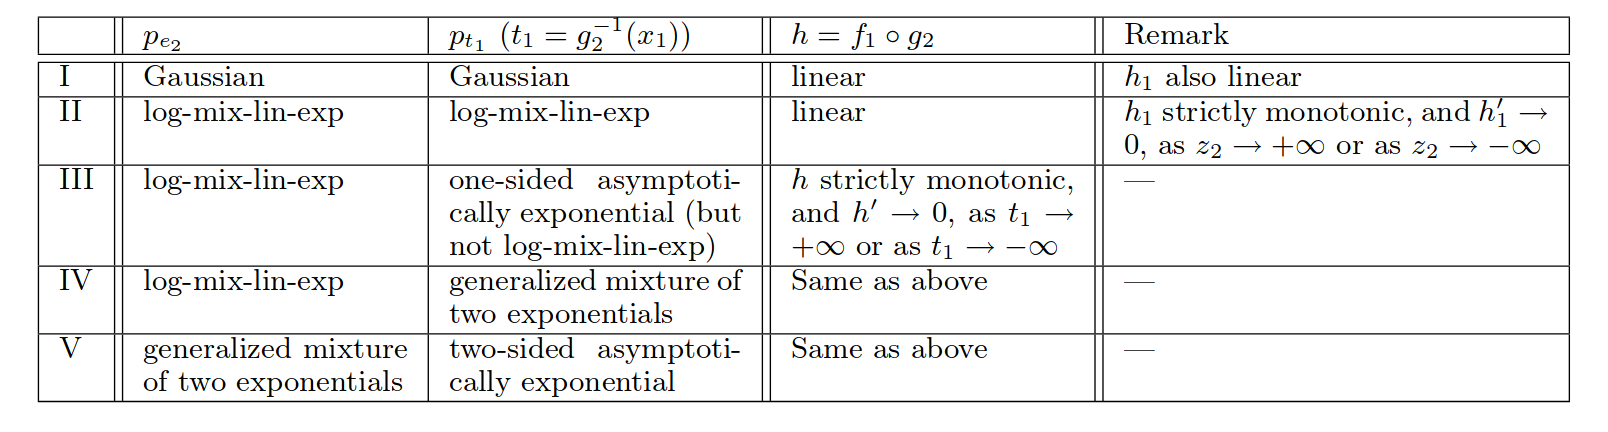
\includegraphics[scale=0.2]{PNL.png}
	\caption{All unidentifiable cases with the assumptions made above}
\end{figure}
\end{frame}

\section{Learning Algorithms}
\subsection{Score Based Method}
\begin{frame}
\frametitle{Score Based Method}
\end{frame}



\subsection{RESIT}
\begin{frame}
\frametitle{RESIT Algorithm}
\begin{itemize}
	\item First proposed in \cite{continous}
	\item Assumption : Multivariate ANM + Causal Sufficiency 
	 \item Idea :  $X_i \textrm{ is sink} \iff N_i \bigCI \mathbf{X} \setminus \{X_i\}$ 
	\item The are two stages in the algorithm:
		\begin{itemize}
			\item Stage 1 : Finding a causal order 
			\item Stage 2 : Estimating DAG by removing edges
		\end{itemize}
	\item Number of Tests (Less than PC)
		\begin{itemize}
			\item Stage 1 : $O(n^2)$			
			\item Stage 2 : $O(n)$
		\end{itemize}
\end{itemize}
\end{frame}

\begin{frame}
\frametitle{RESIT Algorithm}
\begin{figure}
	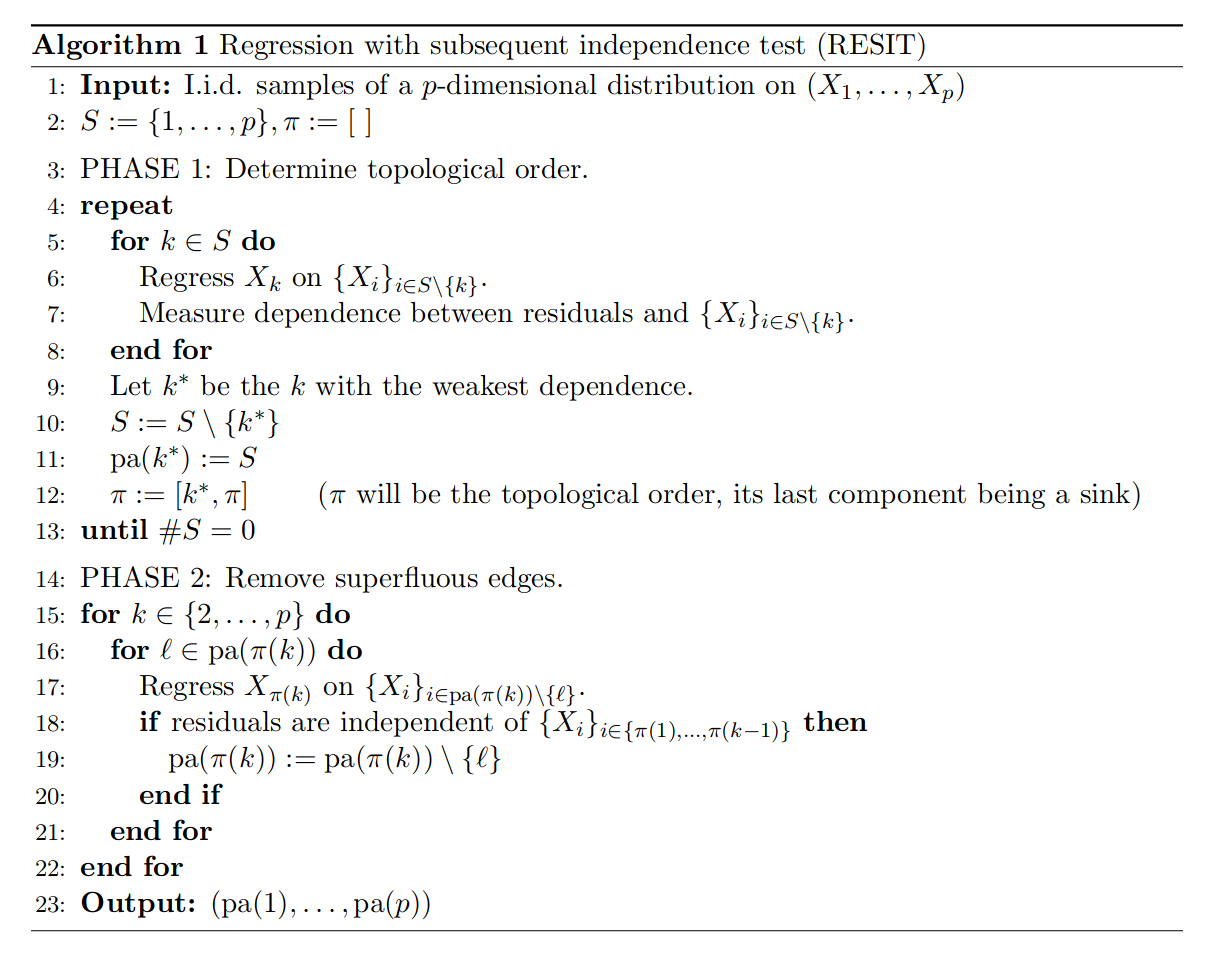
\includegraphics[scale=0.2]{alg.png}
\end{figure}
\end{frame}

\begin{frame}
\frametitle{RESIT Algorithm : Performance (Linear Setting)}
\begin{center}
\scriptsize{$\beta_{jk} \stackrel{}{\sim} [-2,-0.1] \cup [0.1,2]$
$\;\;\;\;\;N_j \stackrel{}{\sim} K_j \cdot \mathrm{sign}(M_j)\cdot |M_j|^{\alpha_j}$
such that
$M_j \stackrel{}{\sim} N(0,1)$, $K_j \stackrel{}{\sim} U(0.1,0.5)$ 
and
$\alpha_j \stackrel{}{\sim} U([2,4])$. }
\end{center}
\begin{figure}[h!]
	\centering
	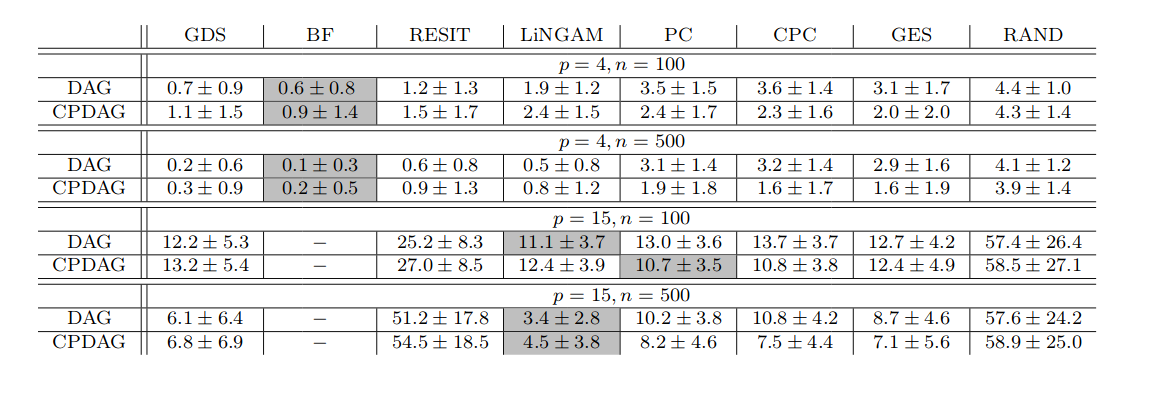
\includegraphics[scale=0.28]{linear.png}
	\caption{Structural Hamming Distance of Estimated Graph}
\end{figure}
\end{frame}

\begin{frame}
\frametitle{RESIT Algorithm : Performance (Non Linear Setting)}
\begin{center}
	\scriptsize{
		Functions sampled from a Gaussian process with $BW=1$. Gaussian Noise with random variance.
	}
\end{center}
\begin{figure}[h!]
	\centering
	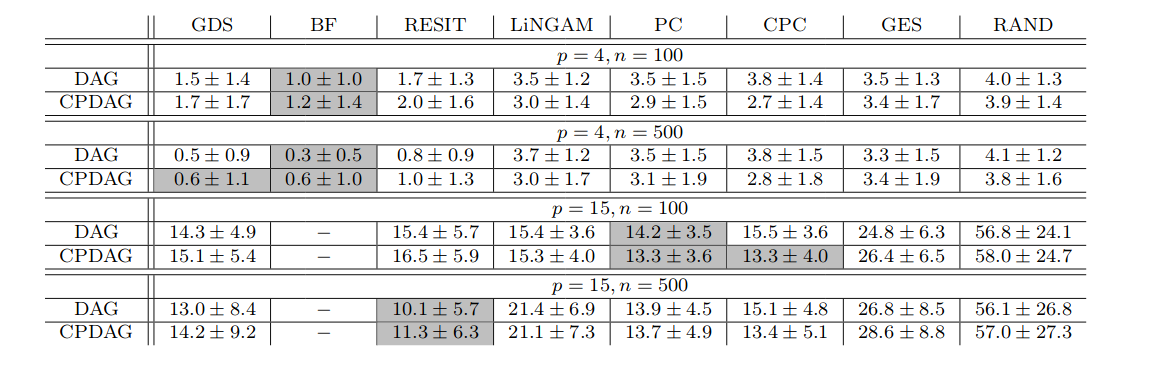
\includegraphics[scale=0.28]{dif.png}
	\caption{Structural Hamming Distance of Estimated Graph}
\end{figure}
\end{frame}
\section{Hidden Variables}
\section{Time Series}
\begin{frame}
\frametitle{References}
\bibliographystyle{plainnat}
\bibliography{bib}
\end{frame}
%------------------------------------------------

\begin{frame}
\Huge{\centerline{The End}}
\end{frame}

%----------------------------------------------------------------------------------------

\end{document}
